\recipe{Halloumi, Broccoli \& Chickpea Curry}
\label{recipe:halloumi_broccoli_chickpea_curry}
\makes{Makes 4 portions}
\worktime{40 minutes}
\totaltime{60 minutes}
\source{\href{https://www.tamingtwins.com/halloumi-curry/}{tamingtwins.com/halloumi-curry}}

\begin{ingredients}
	\item \SI{2}{\tablespoon} Cornflour
	\item \SI{2}{\tablespoon} Sunflower oil
	\item 1 Onion, Halved and sliced
	\item 1 head (\SI{300} \gram) Broccoli cut into small florets
	\item \SI{3}{\tablespoon} Curry paste of your choice
	\item 1 can (\SI{400} \gram) Coconut Milk
	\item 1 can (\SI{400} \gram) Chickpeas, drained
	\item To serve: Naan bread or rice
\end{ingredients}

\begin{method}
In a small bowl, mix the halloumi with the cornflour and toss well to coat.

Heat the oil in large frying pan over a high heat and add the cheese cubes.

Cook over a high heat for 5 minutes until nicely coloured all over.

Remove from the frying pan and set aside on a plate. Add the onion and broccoli to the empty pan (if your pan is not non stick you may need to add a little more oil here).

Cook for 5 minutes until they are starting to soften.

Add the curry paste and stir for 1 minute.

Next, add the coconut milk and chickpeas and bring to a simmer for 10 minutes until everything is mixed and the chickpeas are hot and the broccoli is cooked through.

Add the halloumi back to the pan and stir.

Serve with naan bread.

\end{method}

\begin{figure}[h]
  	\centering
  	
  	\begin{tikzpicture}
  		% Save the image in a box to get its dimensions
  		\sbox0{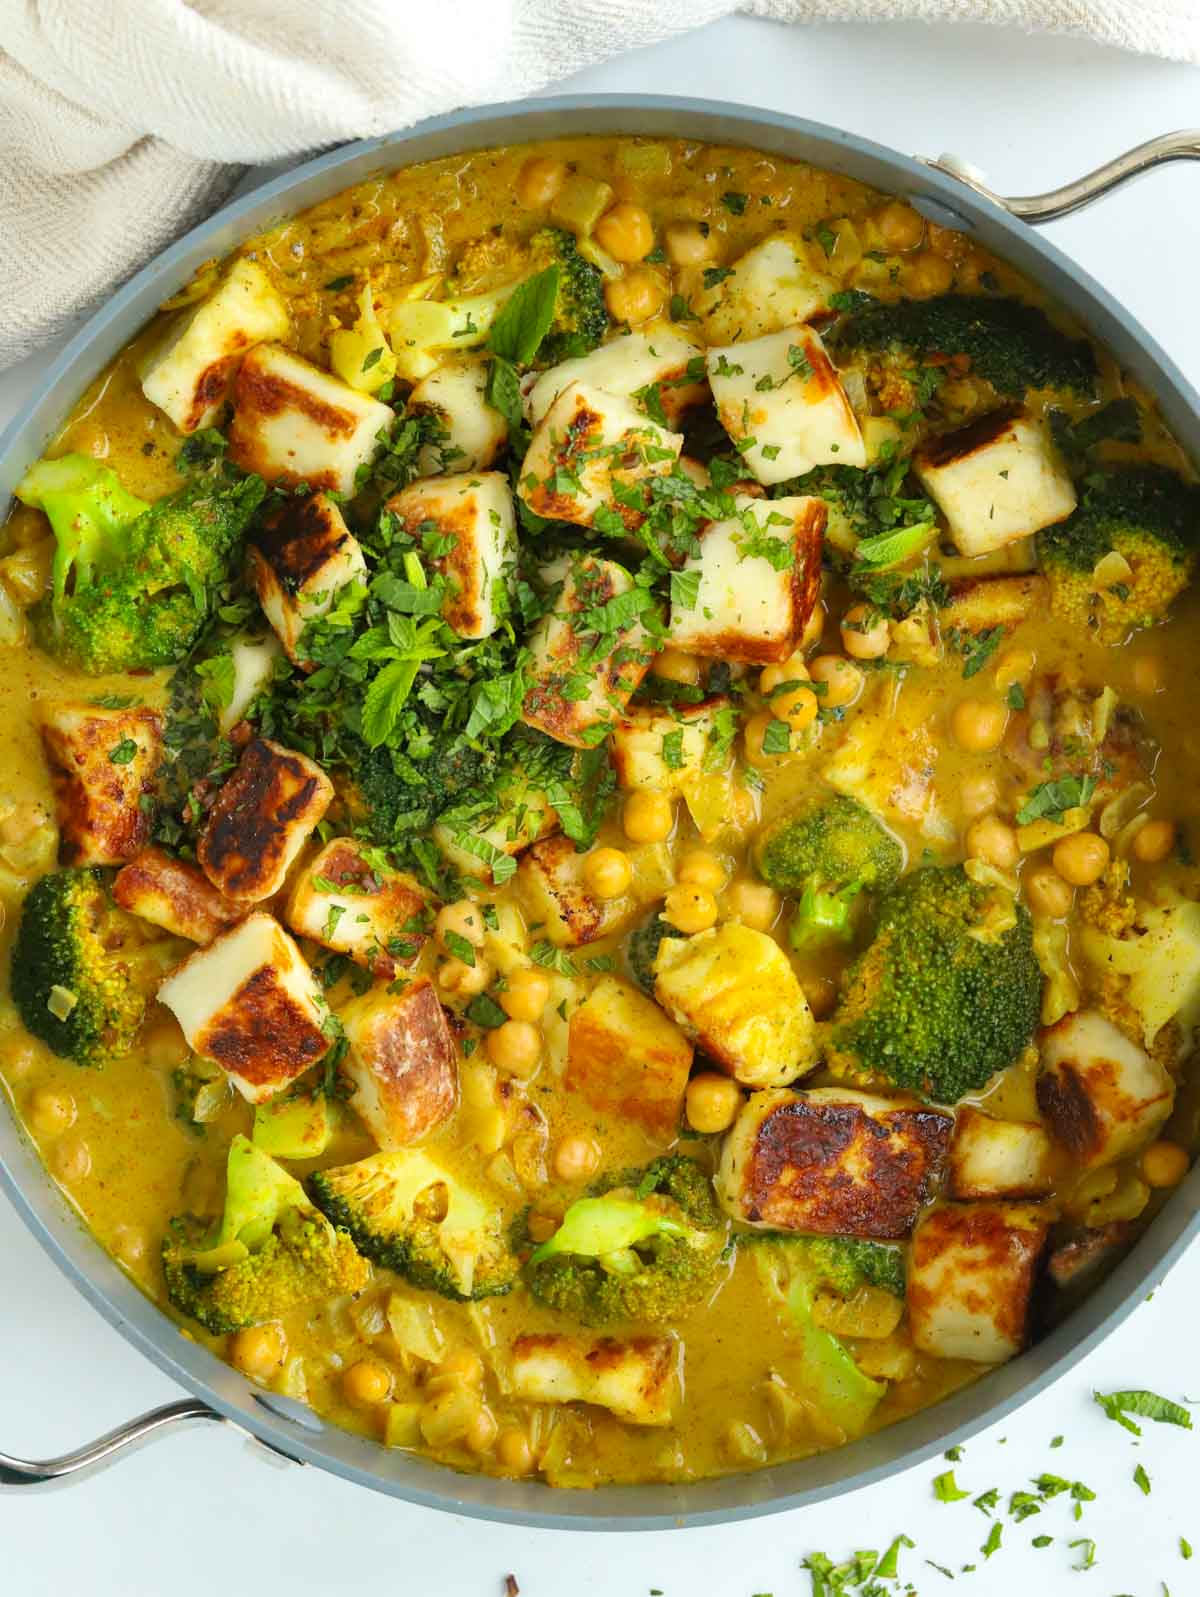
\includegraphics[width=\linewidth]{images/halloumicurry.png}}%
  
  		% Draw a clipping rectangle with rounded corners
  		\path[clip, rounded corners=0.5cm] (0,0) rectangle (\wd0,7cm);
  
  		% Place the image inside the clipped area
  		\node[inner sep=0pt, outer sep=0pt, anchor=south west] at (0,-1cm) {\usebox0};
	\end{tikzpicture}

  \caption*{}
\end{figure}
